
%(BEGIN_QUESTION)
% Copyright 2013, Tony R. Kuphaldt, released under the Creative Commons Attribution License (v 1.0)
% This means you may do almost anything with this work of mine, so long as you give me proper credit

A technician needs to calculate the appropriate length of cable to install computer network wiring in the foundation of a new building.  The dimensions shown on the foundation blueprint are all the technician has to work with:

$$\includegraphics[width=15.5cm]{i03380x01.eps}$$

Calculate the total cable length necessary for this job, as well as the value of the unknown angle shown on the blueprint.

\vskip 20pt

Total cable length = 

\vskip 10pt

$\theta$ = 

\underbar{file i03380}
%(END_QUESTION)





%(BEGIN_ANSWER)

Total cable length = 65 ft

\vskip 10pt

$\theta$ = 30$^{o}$

%(END_ANSWER)





%(BEGIN_NOTES)

{\bf This question is intended for exams only and not worksheets!}.

%(END_NOTES)


